\documentclass{article}
% --- watermark (auto-inserted) ---
\usepackage{xcolor}
\usepackage{xfp}% \fpeval; in the kernel since 2022, harmless on older LaTeX
\usepackage{draftwatermark}
\newlength{\watermarkTextWidth}
\AddToHook{begindocument/end}{%
  \SetWatermarkText{\normalfont Generated by The Agentic Scientist}%
  \SetWatermarkFontSize{10pt}%
  \SetWatermarkLightness{0.85}%
  \settowidth{\watermarkTextWidth}{\normalfont\fontsize{10pt}{12pt}\selectfont Generated by The Agentic Scientist}%
  \edef\watermarkScale{\fpeval{0.8 * sqrt(\paperwidth**2 + \paperheight**2) / \watermarkTextWidth}}%
  \edef\watermarkAngle{\fpeval{atand(\paperheight/\paperwidth)}}%
  \SetWatermarkScale{\watermarkScale}%
  \SetWatermarkAngle{\watermarkAngle}%
}
% --- end watermark ---
\usepackage{iclr2026_conference,times}
\usepackage{amsmath,amssymb,booktabs,graphicx,subcaption}
\usepackage{hyperref,url}
\newcommand{\E}{\mathbb E}
\newcommand{\Var}{\operatorname{Var}}
\newcommand{\Cov}{\operatorname{Cov}}
\newcommand{\R}{\mathbb R}
\title{Risk-Adaptive Frozen-Score Controls:\\Conditional Efficiency in Mean Inference}
\author{}
\begin{document}
\maketitle

\begin{abstract}
Can confidence intervals be shortened without acquiring labels, enlarging the unlabeled sample, or changing a pretrained predictor? We study mean inference using a fixed scalar score, with training-only selection among zero, affine, and nonlinear controls, cross-fitted correction, and a studentizer that accounts for the shared unlabeled sample. Deterministic variance identities explain possible nonlinear gains but do not certify the learned procedure. In a completed assessment with 400 paired repetitions in each of seven conditions, the frozen method reduces mean width on an empirical gene-expression source from 0.4759 for PPI++ to 0.4488, a 5.69\% reduction. It is wider than PPI++ in all six other conditions, including the nonlinear synthetic condition. Its observed condition-wise coverage ranges from 95\% to 98\%, but simultaneous uncertainty intervals do not establish nominal coverage. Rare-outcome comparisons also expose zero-width reference intervals. The evidence supports a conditional efficiency result, not universal narrowing, component-level causal attribution, or a finite-sample validity certificate.
% @evidence[[paper_data.json#final_evaluation/evaluation_evidence/episodes]]
% @evidence[[analysis_summary.json]]
\end{abstract}

\section{Introduction}
Scientific prediction and scientific inference solve different problems. A predictor can be highly useful for assigning scores to observations while remaining biased for a population average. Conversely, a small labeled sample can support an unbiased mean estimate but an imprecise confidence interval. Prediction-powered inference (PPI) combines a large sample of predictions with a labeled correction, retaining the inferential target rather than treating predictions as ground truth \citep{PPI}. Its efficiency depends on the relationship between the labels and the available scores, not simply on the availability of a large prediction table.

We investigate the fixed-resource version of this problem. Within each comparison, every method receives exactly the same labeled outcomes, corresponding scalar predictions, and unlabeled predictions. There is no new label acquisition, predictor retraining, or enlarged prediction pool. The target is the population mean. This setting isolates a practical question: can postprocessing an existing score yield narrower intervals than both the original PPI correction and the power-tuned PPI++ reference \citep{PPIPlus}, without mistaking an empirical width reduction for a guarantee of validity?

The method studied here learns a small control function of the frozen score. It uses outer held-out folds for the mean correction and inner folds to compare zero, affine, and nonlinear calibrations. Its variance estimate centers labeled residuals within folds and evaluates the weighted sum of all fold controls on the single shared unlabeled pool. The construction is motivated by an elementary distinction: an affine rescaling can correct a score's scale, but cannot in general recover a nonlinear conditional mean. Nevertheless, estimating that nonlinear relationship from scarce labels can consume the potential gain. Oracle headroom is therefore a rationale to investigate, not evidence of realized benefit.

Our contribution is a delimited construction and matched empirical assessment. On the empirical gene-expression source, the frozen method is narrower than label-only inference, PPI, and PPI++. Against PPI++, however, none of the other evaluated conditions benefits. Across the assessment, measured coverage is compatible with nominal coverage but too uncertain to establish it. We make the unfavorable comparisons part of the central result rather than treating them as peripheral failures.
% @evidence[[paper_data.json#final_evaluation/evaluation_evidence/episodes/0/solution/summary]]

The study thus contributes an inspectable score-only implementation, an explanation of its variance target and additive-offset invariance, and a comparison that separates efficiency, uncertainty, and validity. No controlled component ablation is available, so we do not attribute the empirical-source gain specifically to nonlinear calibration or to studentization. The operative conclusion is conditional: recalibration can help on the measured source, while improving over an already tuned reference is substantially harder than improving over an unweighted correction.

\begin{figure}[t]
\centering
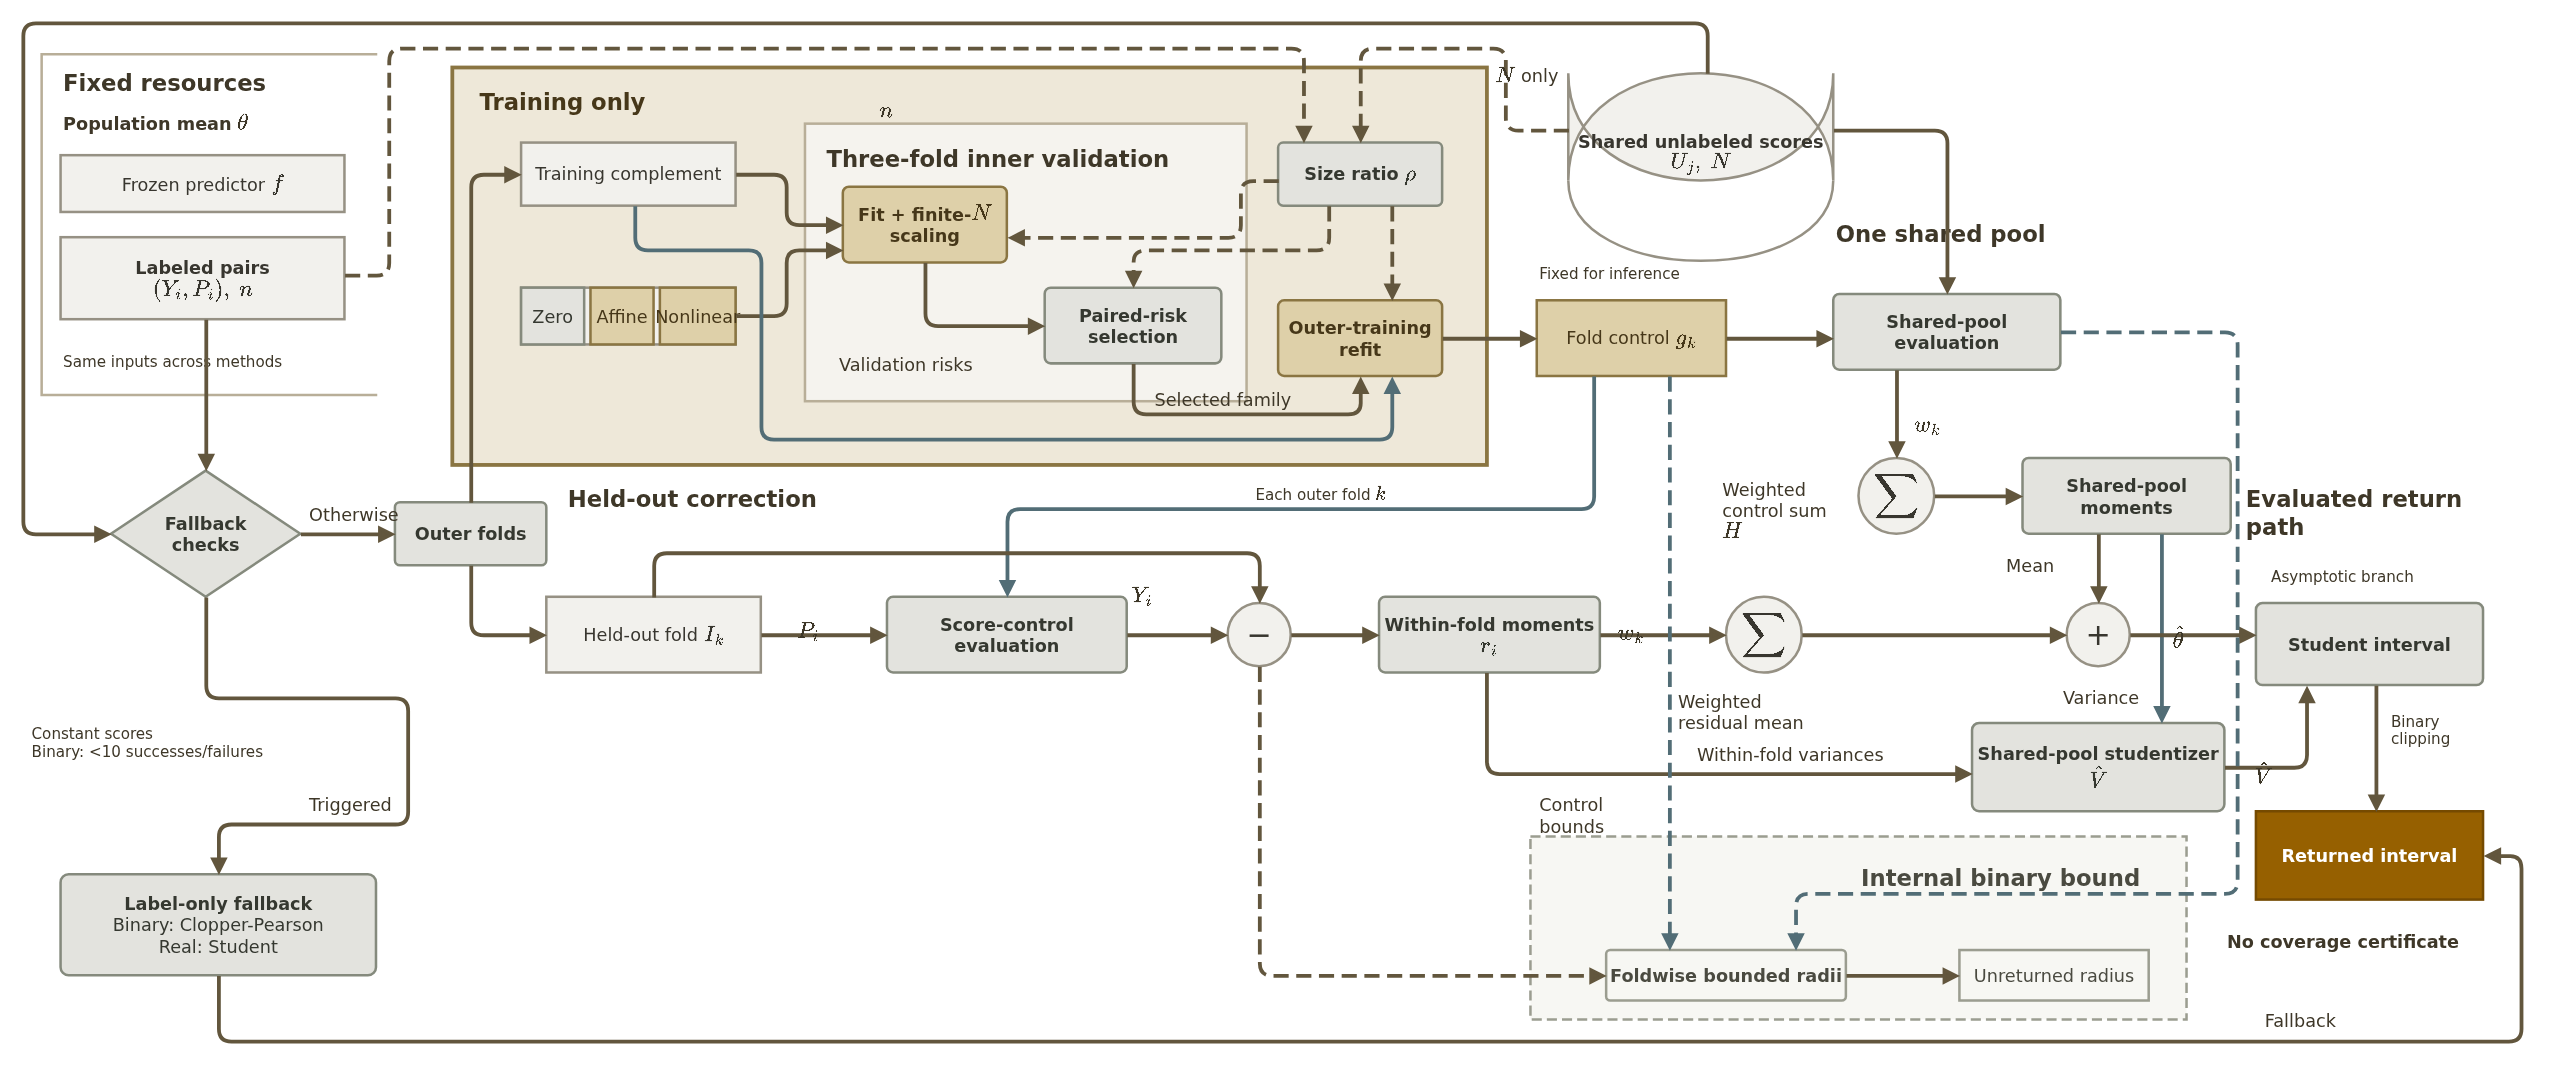
\includegraphics[width=\textwidth]{figures/fixed_resource_overview.png}
\caption{Fixed-resource mean inference. The training boundary separates selection of a score control from the labels used for its held-out correction. Fold controls share one unlabeled sample; inference uses their weighted aggregate rather than independent copies of that sample. The returned asymptotic interval and its repeated-sampling assessment are distinct from an internal bounded construction that is not returned. No arrow denotes a validity certificate.}
\label{fig:overview}
% @evidence[[source_evidence/program.py#L154-L305]]
\end{figure}

\section{Related Work}
\paragraph{Correction and efficiency.}
PPI \citep{PPI} supplies the prediction-plus-correction framework; PPI++ \citep{PPIPlus} makes power tuning an essential comparator rather than a cosmetic implementation choice. The present study does not replace either framework with a new inferential target. It considers a restricted learned transformation of an externally frozen scalar score. Cross-prediction \citep{CrossPPI} addresses inference when prediction itself is learned with the available labels. Here only the calibration is learned; the upstream predictor remains fixed. Cross-fitting and orthogonal correction also have a broader role in debiased inference \citep{DML}, but that connection does not automatically verify assumptions for a particular selected calibration.

\paragraph{Controls and model-assisted means.}
The control-variate perspective \citep{Glynn}, generalized difference estimation \citep{Cassel}, and model-assisted sampling \citep{Sarndal} motivate correcting a prediction-based mean with observed residuals. Semi-supervised mean inference explicitly studies how finite unlabeled information changes efficiency \citep{Zhang}. Empirical efficiency maximization \citep{Rubin} provides related motivation for selecting an adjustment by variance rather than prediction error alone. These connections explain why our inner objective contains both residual variability and a finite-unlabeled-sample penalty. They do not identify the present procedure as optimal over all estimators or all interval constructions.

\paragraph{Learning and inferential boundaries.}
The low-dimensional calibration uses ridge regularization \citep{Hoerl} and elementary basis expansion \citep{Hastie}. Held-out selection follows the general cross-validation principle \citep{Stone}; dependence among reused training sets complicates uncertainty assessment \citep{Nadeau}. Out-of-fold prediction also appears in stacked generalization and stacked regression \citep{Wolpert,Breiman}, but our measured method selects one control family per outer fold rather than fitting a stack. For uncertainty reporting, exact binomial intervals \citep{ClopperPearson} and the known pitfalls of normal binomial approximations \citep{Brown} are particularly relevant to rare outcomes. Bounded concentration \citep{Hoeffding,MaurerPontil} is conceptually different from the Student-based interval returned here. Keeping these distinctions explicit is necessary for interpreting a width advantage scientifically.

\section{Method}
\subsection{Problem setup and fixed resources}
Let $(Y_i,P_i)_{i=1}^{n}$ be independent, identically distributed labeled pairs and $(U_j)_{j=1}^{N}$ an independent sample from the same marginal score distribution. The scalar score is $P=f(X)$ for an externally frozen predictor. We estimate $\theta=\E[Y]$. The inferential objective is a short interval $I$ satisfying $\Pr\{\theta\in I\}\geq 1-\alpha$ under repeated sampling. Fixing resources means holding the realized inputs equal \emph{across methods}, not asserting coverage conditional on the entire realized labeled sample. Informative label selection, predictor training on these labels, and a shifted unlabeled population require additional justification and are outside this setup.
% @evidence[[source_evidence/METHOD.md#L12-L28]]

For any deterministic score control $g$ with finite second moments, consider
\begin{equation}
 \widehat\theta_g=\frac1n\sum_{i=1}^n\{Y_i-g(P_i)\}
             +\frac1N\sum_{j=1}^Ng(U_j).
 \label{eq:control}
\end{equation}
The correction removes the mean bias of $g$, so $g$ need not be an unbiased predictor. Setting $g=0$ gives the labeled mean, while $g(p)=p$ gives the unweighted PPI point estimate. A tuned linear multiple yields the corresponding scalar power-tuned family. Our rationale is to enlarge this control class slightly without spending additional observations or modifying $f$.
% @evidence[[source_evidence/METHOD.md#L108-L143]]

\subsection{Training-only risk adaptation}
The implementation divides a seeded permutation of the labeled indices into $K=\min(5,\lfloor n/2\rfloor)$ outer folds. For each held-out fold, its complement supplies all calibration and selection data. Three inner validation folds are shared across the candidate families. The zero control provides an anchor; the affine fit learns a scalar least-squares slope and intercept; the nonlinear fit uses a linear term, a quadratic term, and positive-part terms with normalized knots $-0.5,0,0.5$. Training-score quantiles determine normalization. The diagonal ridge penalties are $(0.1,2,4,4,4)$. Binary calibration predictions, before the multiplier below, are clipped to $[0,1]$.
% @evidence[[source_evidence/program.py#L69-L211]]

For a fitted calibration $q$ and $\rho=n/N$, its training-only multiplier is
\begin{equation}
 b=\frac{\widehat\Cov(Y,q(P))}{(1+\rho)\widehat\Var(q(P))},
 \qquad g(p)=bq(p).
 \label{eq:weight}
\end{equation}
Degenerate or nonfinite denominators give the zero control. Multipliers can be signed; clipping $q$ does not restrict $g$ to a probability. On inner validation fold $v$, the criterion is
\begin{equation}
 J_v(g)=s_v^2\{Y-g(P)\}+\rho s_v^2\{g(P)\}.
 \label{eq:risk}
\end{equation}
Starting from zero, the implementation compares affine and nonlinear controls in increasing complexity. A challenger replaces the retained family only when the mean paired excess risk plus its standard error across the inner folds is negative. The selected family is refitted on the entire outer training complement. This is a conservative heuristic relative to selecting the smallest observed risk, not a calibrated significance test: inner training sets overlap, and three folds do not supply independent risk replicates. The unlabeled score values enter neither normalization nor fitting nor this selection rule; only their sample size enters $\rho$.
% @evidence[[source_evidence/program.py#L154-L211]]

\subsection{Held-out correction and shared-pool studentization}
For outer fold $\mathcal I_k$, write $n_k=|\mathcal I_k|$, $w_k=n_k/n$, and let $g_k$ be its fitted control. Define $r_i=Y_i-g_k(P_i)$ for $i\in\mathcal I_k$ and $H(u)=\sum_k w_kg_k(u)$. The estimate and estimated variance are
\begin{align}
 \widehat\theta&=\sum_k w_k\overline r_k+\overline H_U,\label{eq:crossfit}\\
 \widehat V&=\sum_k\frac{w_k^2}{n_k}s_k^2(r)
                        +\frac{s_U^2(H)}{N}.\label{eq:studentizer}
\end{align}
Here $s^2$ denotes sample variance with the usual degrees-of-freedom correction. The unlabeled term is the variance of a weighted \emph{sum} of predictions evaluated on the same observations. Treating foldwise unlabeled means as independent would drop their covariance. Centering residuals within folds also avoids treating fold-specific prediction offsets as between-observation residual variation.
% @evidence[[source_evidence/program.py#L215-L267]]

For the nonfallback return, the radius is $t_{1-\alpha/2,\,\max(2,n-6)}\sqrt{\max(0,\widehat V)}$. Binary endpoints are clipped to $[0,1]$. Constant scores in either pool trigger label-only inference. For binary outcomes, fewer than ten successes or fewer than ten failures also trigger that fallback: a Clopper--Pearson interval. The real-valued fallback uses a Student interval \citep{Student}. Its exactness requires Gaussian outcomes, not merely real-valued measurements. These details matter when comparing widths: reference methods need not share the same critical value, variance convention, or fallback behavior.
% @evidence[[source_evidence/program.py#L270-L305]]

An internal bounded-fold construction is also computed for binary inputs, but does \emph{not} determine the returned interval. We therefore do not credit its concentration argument to the empirical intervals. Similarly, the presence of an exact binomial fallback does not make the full data-dependent fallback/Wald rule finite-sample exact. Figure~\ref{fig:overview} separates these objects. Readable implementation evidence is included as \path{source_evidence/program.py}, with the accompanying \path{source_evidence/METHOD.md}; source locations and the reference implementation are indexed in the supplement.

\section{Variance Rationale and Validity Boundaries}
\subsection{Oracle headroom is conditional}
For a common deterministic $g$, independence gives
\begin{equation}
 V(g)=\frac{\Var\{Y-g(P)\}}{n}+\frac{\Var\{g(P)\}}{N}.
\end{equation}
Let $m(P)=\E[Y\mid P]$, $e=\E[\Var(Y\mid P)]$, and $a=N/(n+N)$. Orthogonality of $Y-m(P)$ to functions of $P$ and completion of the square yield
\begin{equation}
 V(g)=\frac{e}{n}+\frac{\Var(m)}{n+N}
       +\left(\frac1n+\frac1N\right)\Var(g-am).
 \label{eq:oracle}
\end{equation}
Thus $am$, up to an additive constant, minimizes variance within this deterministic control family. The finite-$N$ multiplier is not optional when the unlabeled mean itself has sampling error. This identity does not optimize interval length over arbitrary confidence procedures.
% @evidence[[source_evidence/METHOD.md#L119-L143]]

For $\Var(P)>0$, the best affine control has variance
\begin{align}
 V_{\mathrm{aff}}&=\frac{\Var(Y)}n-
 \frac{N\Cov(Y,P)^2}{n(n+N)\Var(P)},\\
 V_{\mathrm{aff}}-V_{\mathrm{oracle}}
 &=\frac{N}{n(n+N)}\left\{\Var(m)-\frac{\Cov(Y,P)^2}{\Var(P)}\right\}.\label{eq:headroom}
\end{align}
The gap vanishes for an affine conditional mean, an uninformative score, or a score supported on at most two values. For an independently fixed calibration $\widehat m$, the corresponding risk identity is
\begin{equation}
 nV(a\widehat m)=\Var(Y)-a\Var(m)+a\Var(\widehat m-m).
 \label{eq:calibration}
\end{equation}
Even positive nonlinear headroom can be lost to calibration error. These identities motivate the zero and affine anchors, but they neither predict the measured ranking in every condition nor prove that the selected nonlinear basis learns $m$. In particular, an evaluated condition bearing a nonlinear response does not guarantee a width benefit over PPI++.
% @evidence[[source_evidence/METHOD.md#L119-L143]]

\subsection{What the studentizer establishes}
For deterministic, possibly different $g_k$, the exact variance of Eq.~\eqref{eq:crossfit} is
\begin{equation}
 \sum_k\frac{w_k^2}{n_k}\Var\{Y-g_k(P)\}
  +\frac1N\Var\!\left\{\sum_k w_kg_k(P)\right\}.
 \label{eq:fixedfold}
\end{equation}
Equation~\eqref{eq:studentizer} estimates this expression without omitting shared-pool covariance. Moreover, replacing $g_k$ by $g_k+c_k$ subtracts $\sum_kw_kc_k$ from the labeled center and adds the same constant to the unlabeled center. Every variance term is unchanged. Both endpoints are therefore invariant to fold-specific additive shifts, provided shifted controls are not reclipped. This is an algebraic property, not evidence that the empirical widths necessarily decrease.
% @evidence[[source_evidence/METHOD.md#L80-L117]]

With learned $g_k$, overlapping training complements create dependence. Conditioning jointly on all fitted controls does not make the held-out labeled terms independent. A sufficient asymptotic route is fixed $K$, $n,N\to\infty$ with $N/n$ tending to a positive finite constant, finite $2+\delta$ moments and suitable uniform integrability, nondegenerate limiting variance, and $L^2$ convergence of each control, modulo additive constants, to a common deterministic function. Under these stability conditions, the nuisance-error averages are negligible at first order, giving a common-control central limit approximation and a consistent variance estimate. The inner risk rule does not establish these conditions, especially near ties between distinct controls. Neither the Student critical value nor clipping turns this argument into a finite-sample theorem.
% @evidence[[source_evidence/METHOD.md#L144-L166]]

\section{Evaluation Design}
\subsection{Conditions, targets, and matched inputs}
The final assessment contains 400 seeded repetitions for each of seven conditions, using $n=128$ labels and $N=8192$ unlabeled scores at nominal coverage $0.95$. Seeds range from 1000 through 1399. Every paired method sees identical inputs. The synthetic resources specify independent uniform scalar scores with Bernoulli outcomes; the recorded targets are $0.5$ for the linear and uninformative conditions, $0.1+0.8/3$ for the nonlinear condition, and $0.01+0.08/3$ for rare outcomes. These are the evaluator's population targets, not empirical labeled means. We analyze the archived draws; no additional simulation or evaluation was performed during manuscript preparation.
% @evidence[[paper_data.json#final_evaluation/evaluation_evidence/episodes]]
% @evidence[[source_evidence/evaluate_final.py#L861-L895]]
% @evidence[[source_evidence/resource_manifest.json#raw_shapes]]

The empirical condition uses the gene-expression example distributed with the fixed PPI reference release, whose source attribution is \citet{Vaishnav}. Normalized duplicate outcome--score records are grouped before a deterministic development/final partition. Labeled and unlabeled observations are sampled independently with replacement from the final unique-record source. Consequently, its truth is the mean of that empirical source, not a claim about all promoter sequences or a new biological population. Underlying sequence strings are unavailable, so disjointness of normalized scalar records does not establish sequence-level disjointness.
% @evidence[[source_evidence/resource_manifest.json#source]]
% @evidence[[source_evidence/evaluate_final.py#L861-L873]]

The remaining information controls use the nonlinear outcomes unchanged. Constant scores replace both prediction pools by $0.5$; permuted scores separately permute the labeled and unlabeled predictions. The latter intervention disrupts label--score pairing while retaining each prediction multiset. These conditions test reliance on information, not isolated contributions of studentization or nonlinear fitting. They share records with the nonlinear condition and must not be counted as independent natural datasets.
% @evidence[[source_evidence/evaluate_final.py#L885-L893]]

\subsection{References, uncertainty, and assessment scope}
The label-only reference uses exact binomial intervals for binary data and Student intervals for real data. PPI and PPI++ use \texttt{ppi-python==0.2.3}, with respectively \texttt{lam=1} and \texttt{lam=None}. The latter estimates a coefficient clipped to $[0,1]$ and uses pooled prediction variance. On constant scores it uses coefficient zero. Both references return normal-approximation intervals; their finite-sample behavior should not be inferred from asymptotic theory alone.
% @evidence[[source_evidence/evaluate_final.py#L754-L809]]
% @evidence[[source_evidence/ppi.py#L135-L229]]

Coverage is computed from recorded interval endpoints and the evaluator's target. The stored coverage intervals are Clopper--Pearson intervals with Bonferroni allocation over seven conditions and four methods, giving joint coverage of at least $95\%$ under the repetition model. They quantify Monte Carlo uncertainty, not uncertainty about $\theta$ within a repetition. Dependence between information-control conditions does not invalidate the union bound. Width comparisons use the stored paired bootstrap with 512 seed resamples and random seed 79231. The percentile endpoints use tail probability $0.05/42$ for the seven-by-three comparison family. These are multiplicity-adjusted bootstrap summaries, not exact simultaneous confidence guarantees \citep{Efron,EfronTibshirani,Dunn}.
% @evidence[[source_evidence/evaluate_final.py#L920-L974]]

We report the ratio of mean widths, not the mean of per-repetition ratios. This distinction avoids zero-denominator sensitivity. The assessment's secondary aggregate caps per-repetition ratios at 100; we do not interpret that capped aggregate as a typical percentage increase. All final repetitions are retained, with no recorded failures or missing paired intervals. Operational and information-control qualification completed successfully, but the evaluator explicitly does not certify arbitrary theoretical variance assumptions. This completed qualification is not a coverage theorem. Selection used development evidence; final measurements and descriptive source inspection are kept separate from that selection history.
% @evidence[[paper_data.json#final_evaluation]]
% @evidence[[source_evidence/resource_manifest.json#scientific_limits]]

\section{Results}
\subsection{A localized empirical-source efficiency gain}
Table~\ref{tab:main} and Figure~\ref{fig:width} give matched comparisons for every condition. Gene expression provides the sole width advantage over PPI++: the frozen method has mean width $0.448807$, compared with $0.475901$ for PPI++, $0.472748$ for PPI, and $1.526381$ for label-only inference. The ratio to PPI++ is $0.94307$, a $5.69\%$ mean-width reduction. The paired difference interval is $[-0.029691,-0.024356]$. Thus the observed improvement over the tuned reference is small compared with the difference from ignoring predictions, but it remains separated from zero in the stored bootstrap summary.
% @evidence[[paper_data.json#final_evaluation/evaluation_evidence/episodes/0/solution/summary/gene_expression]]
% @evidence[[analysis_summary.json#conditions/gene_expression]]

The result is about these evaluated configurations on this empirical source. It does not show that nonlinear calibration caused the gain: the frozen method also changes fitting, fold aggregation, variance estimation, and return behavior relative to the references. Selection frequencies and fold-specific calibration outputs are not available as trusted final diagnostics. Without an affine-only matched assessment and a controlled studentizer comparison, the width result cannot distinguish these explanations. The oracle identities supply an interpretation of possible headroom, not a retrospective mechanism label.

\begin{table}[t]
\centering
\small
\caption{Final paired results. Widths are means over 400 repetitions in each condition. Ratios divide the frozen method's mean width by PPI++ mean width. Coverage is the frozen method's observed coverage; simultaneous uncertainty is displayed in Figure~\ref{fig:coverage}. Width units differ between real-valued gene expression and binary conditions, so raw widths should not be averaged across rows.}
\label{tab:main}
\begin{tabular}{lrrrrrr}
\toprule
 & \multicolumn{4}{c}{Mean interval width} & Ratio & Coverage\\
Condition & Frozen & Label only & PPI & PPI++ & to PPI++ & Frozen\\
\midrule
Gene expression & .448807 & 1.526381 & .472748 & .475901 & .9431 & .9575\\
Linear & .156954 & .178575 & .154546 & .152838 & 1.0269 & .9575\\
Nonlinear & .149929 & .172818 & .147968 & .146140 & 1.0259 & .9500\\
Rare outcome & .071556 & .071630 & .112452 & .061507 & 1.1634 & .9800\\
Uninformative & .175416 & .178585 & .199831 & .172244 & 1.0184 & .9575\\
Constant score & .172818 & .172818 & .166680 & .166680 & 1.0368 & .9700\\
Permuted score & .169561 & .172818 & .194657 & .166414 & 1.0189 & .9550\\
\bottomrule
\end{tabular}
% @evidence[[paper_data.json#final_evaluation/evaluation_evidence/episodes]]
% @evidence[[analysis_summary.json]]
\end{table}

\begin{figure}[t]
\centering
\begin{subfigure}[t]{\textwidth}
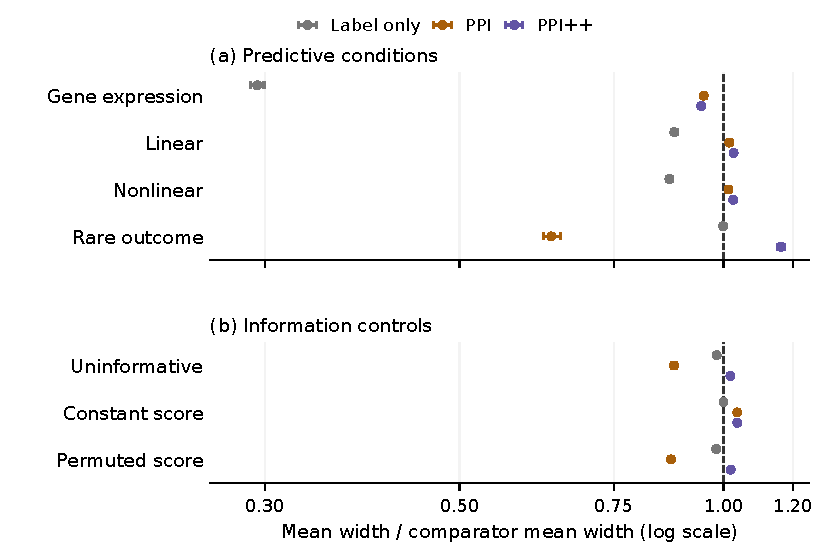
\includegraphics[width=\linewidth,trim=0 120bp 0 0,clip]{figures/paired_width_comparison.pdf}
\phantomsubcaption\label{fig:width-a}
\end{subfigure}\par
\begin{subfigure}[t]{\textwidth}
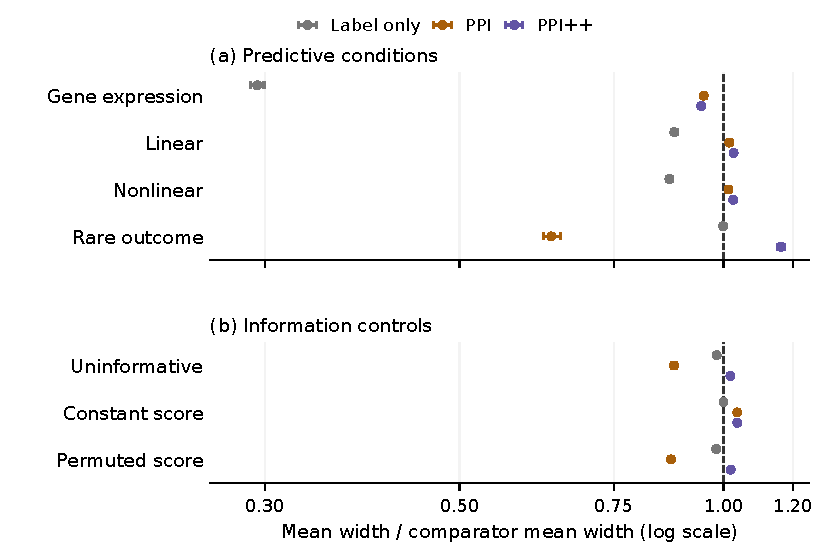
\includegraphics[width=\linewidth,trim=0 0 0 146.4bp,clip]{figures/paired_width_comparison.pdf}
\phantomsubcaption\label{fig:width-b}
\end{subfigure}
\caption{Condition-specific width comparisons. Each point divides frozen-method mean width by the indicated reference mean width; bars are the stored multiplicity-adjusted paired-bootstrap ratio intervals. (a) Predictive conditions. (b) Information controls. Values left of one are narrower, not necessarily more valid. Only gene expression is narrower than PPI++; all six other conditions favor PPI++ on mean width. The rare-outcome comparison requires the coverage and zero-width caveats in the text.}
\label{fig:width}
% @evidence[[paper_data.json#final_evaluation/evaluation_evidence/episodes/0/solution/summary]]
\end{figure}

\subsection{Non-benefits against the tuned reference}
Against PPI++, the frozen method is wider in every non-gene-expression condition. The ratios of means are $1.0269$ for linear, $1.0259$ for nonlinear, $1.1634$ for rare outcomes, $1.0184$ for uninformative scores, $1.0368$ for constant scores, and $1.0189$ for permuted scores. All six stored paired width-difference intervals are strictly positive. The explicitly nonlinear condition is therefore a substantive non-benefit: including a nonlinear basis and positive theoretical headroom does not suffice to improve the measured interval.
% @evidence[[analysis_summary.json]]
% @evidence[[paper_data.json#final_evaluation/evaluation_evidence/episodes/0/solution/summary]]

The baseline distinction is consequential. The frozen method is narrower than label-only inference in the linear, nonlinear, uninformative, and permuted conditions, yet wider than PPI++ in each. It is also narrower than unweighted PPI under uninformative or permuted scores, where applying an untuned score correction can add noise. Neither comparison establishes that the learned procedure extracts useful nonlinear information. Under constant scores it exactly matches the binomial label-only intervals, as the fallback requires. PPI and PPI++ coincide there but are narrower, reflecting different interval constructions rather than predictive information created by a constant score.
% @evidence[[analysis_summary.json]]

\subsection{Coverage uncertainty and the rare-outcome boundary}
The frozen method's condition-wise coverage spans $0.95$ to $0.98$; its equal-condition aggregate is $0.961071$. On gene expression, 383 of 400 intervals cover the empirical-source mean, giving coverage $0.9575$ with stored simultaneous interval $[0.916312,0.982416]$. Every condition's lower bound for the frozen method is below $0.95$. Thus observing at least nominal coverage in these samples does not demonstrate that the underlying coverage probability is at least nominal. Figure~\ref{fig:coverage} keeps all simultaneous bounds visible rather than using a pass/fail color based only on point estimates.
% @evidence[[paper_data.json#final.metric.empirical_coverage]]
% @evidence[[paper_data.json#final_evaluation/evaluation_evidence/episodes]]
% @evidence[[analysis_summary.json]]

Rare outcomes make the efficiency/validity distinction particularly concrete. PPI++ has observed coverage $0.92$ with interval $[0.868958,0.956253]$, which includes nominal coverage. Five of its 400 recorded intervals have zero width. The frozen method has observed coverage $0.98$ and mean width $0.071556$, versus $0.061507$ for PPI++. We retain the narrower reference widths but do not call them a valid practical improvement; conversely, the simultaneous interval does not establish a statistically detected PPI++ coverage shortfall. The evidence shows a finite-sample warning, not a proof of either method's coverage guarantee or superiority.
% @evidence[[paper_data.json#final_evaluation/evaluation_evidence/episodes]]
% @evidence[[analysis_summary.json#conditions/rare_outcome]]

\begin{figure}[t]
\centering
\begin{subfigure}[t]{\textwidth}
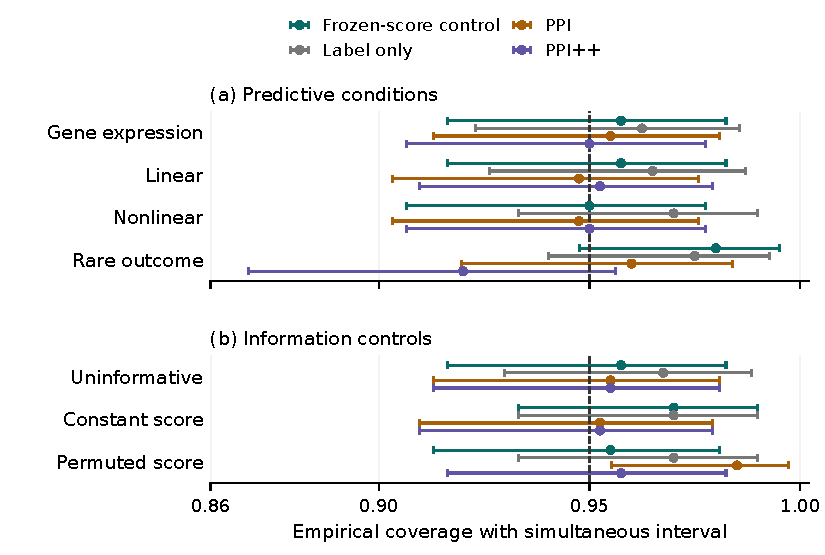
\includegraphics[width=\linewidth,trim=0 120bp 0 0,clip]{figures/coverage_with_uncertainty.pdf}
\phantomsubcaption\label{fig:coverage-a}
\end{subfigure}\par
\begin{subfigure}[t]{\textwidth}
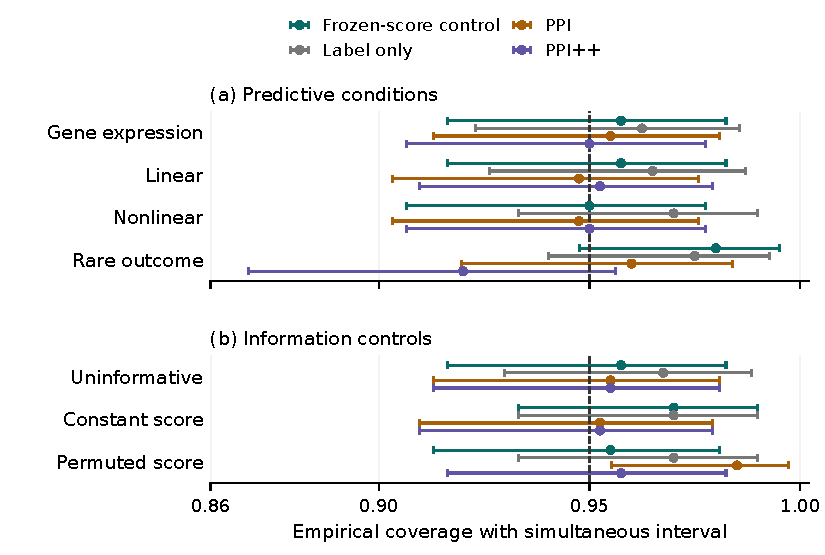
\includegraphics[width=\linewidth,trim=0 0 0 146.4bp,clip]{figures/coverage_with_uncertainty.pdf}
\phantomsubcaption\label{fig:coverage-b}
\end{subfigure}
\caption{Coverage and Monte Carlo uncertainty for all compared methods. Bars are the stored Clopper--Pearson intervals adjusted over all seven conditions and four methods; the dashed line is nominal coverage $0.95$. (a) Predictive conditions. (b) Information controls. Lower bounds for the frozen method remain below nominal throughout. In the rare-outcome condition, PPI++ has the lowest observed coverage, but its interval still contains nominal. These measurements are not finite-sample certificates.}
\label{fig:coverage}
% @evidence[[paper_data.json#final_evaluation/evaluation_evidence/episodes]]
\end{figure}

\section{Discussion and Limitations}
\paragraph{What the comparison answers.}
Holding all observation resources fixed leaves room to change how a score is used. The gene-expression result demonstrates a measured width reduction for the complete frozen procedure relative to the supplied references. The non-benefits show why that observation cannot be promoted to a generally better method. In particular, comparisons with an untuned correction can exaggerate the apparent value of learning a richer calibration. The tuned reference is indispensable for asking whether extra flexibility actually improves interval efficiency.

\paragraph{Validity remains a separate requirement.}
The original goal requires nominal coverage, not simply narrower intervals. The present evidence does not fully discharge that requirement. Deterministic-control variance identities are exact under their assumptions, while the learned-fold argument additionally requires stability and moments. The returned interval is asymptotic, its fallback is selected using the observed outcomes, and a separately computed bounded construction is not its certificate. The completed final qualification confirms the assessment's operational conditions, not these statistical assumptions. We therefore present a conditional efficiency study with an unresolved finite-sample validity boundary, rather than a generally valid interval-shortening solution.
% @evidence[[paper_data.json#final_evaluation/outcome]]
% @evidence[[source_evidence/METHOD.md#L144-L183]]

\paragraph{Identification and external validity.}
There is no controlled component ablation, so neither the role of the nonlinear basis nor the benefit of offset invariance is empirically isolated. The information controls alter the prediction information, not a single inference component. Only one real-valued empirical source is evaluated. Sampling normalized records with replacement gives a well-defined empirical-source estimand, but not a population-level biological validation or sequence-level independence guarantee. Heavy tails, distribution shift, informative labeling, predictor reuse of these labels, alternative sample sizes, and other scientific targets were not evaluated. The synthetic archives permit exact input replay, but the complete generating functions are not provided in the available manifest; we do not reconstruct them from condition names.

\paragraph{Uncertainty and reproducibility.}
The simultaneous binomial intervals are intentionally conservative. The paired bootstrap summarizes the completed repetitions, but its extreme percentile endpoints use a limited resampling budget; it should not be read as an exact simultaneous test. Multiple comparisons and estimator selection are different issues: adjusting result summaries does not validate the inner model-selection rule. Replacing Bonferroni allocation with a stepwise procedure such as \citet{Holm} would change the reporting protocol and is not evaluated here. Finally, the upstream example archive has no separately declared data license in the supplied provenance. Reproduction from available local resources is documented, but redistribution rights require resolution before public release.
% @evidence[[source_evidence/resource_manifest.json#source/license]]
% @evidence[[source_evidence/evaluate_final.py#L920-L974]]

\section{Conclusion}
Risk-adaptive frozen-score controls provide a concrete way to investigate interval efficiency without obtaining more labels, changing a predictor, or enlarging the unlabeled sample. Their variance target clarifies both the potential value of nonlinear calibration and the cost of estimating it. Accounting for a shared prediction pool and preserving fold-offset invariance are useful implementation properties, but neither implies universal narrowing or finite-sample coverage.

The completed matched assessment supports a localized empirical-source result: narrower gene-expression intervals than both PPI references, accompanied by wider intervals than PPI++ in every other evaluated condition. Coverage measurements remain uncertain, and the rare-outcome reference exposes degenerate intervals that prevent a width-only interpretation. The study therefore answers the fixed-resource question conditionally rather than affirmatively in general. Establishing a generally valid shortening rule would require a returned certificate or a fully verified asymptotic regime, stronger coverage evidence, and controlled comparisons separating calibration from studentization. Those are unresolved requirements, not outcomes claimed here.
% @evidence[[paper_data.json#final_evaluation/evaluation_evidence/episodes]]

\clearpage
\bibliography{references}
\bibliographystyle{iclr2026_conference}
\clearpage
\appendix
\section{Supplementary Information}
\subsection{Derivations and the scope of exact identities}
For a deterministic control, write $Y-g(P)=Y-m(P)+m(P)-g(P)$. Conditional mean zero of $Y-m(P)$ makes its covariance with every square-integrable function of $P$ vanish. Hence
\[
 nV(g)=e+\Var(m-g)+\frac nN\Var(g).
\]
Completing the square gives Eq.~\eqref{eq:oracle}; optimizing over an affine slope gives Eq.~\eqref{eq:headroom}. Equation~\eqref{eq:calibration} follows by substituting $g=a\widehat m$. Additive constants are immaterial throughout. These calculations explain a restricted oracle comparison, not an efficiency lower bound over all possible inference procedures. In particular, binary scores support only an affine function of the score, and a constant score offers no nonconstant control in this class.
% @evidence[[source_evidence/METHOD.md#L108-L143]]

For independently fixed fold controls, the unlabeled term in Eq.~\eqref{eq:fixedfold} expands as
\[
 \frac1N\sum_{k,\ell}w_kw_\ell\Cov\{g_k(P),g_\ell(P)\}.
\]
All cross terms are retained by evaluating $H$ before taking its variance. For learned controls, exact unbiasedness of the full estimator can be checked fold by fold under integrability and the stated training boundary, but the deterministic variance expression is not thereby an exact conditional variance formula. Cross-fold labeled dependence remains. A stable common-control limit, rather than joint conditional independence, is the route described in the method note.
% @evidence[[source_evidence/METHOD.md#L108-L166]]

\subsection{Complete coverage and paired differences}
Table~\ref{tab:coverage} supplies observed coverage for every reference. The uncertainty for these points is shown in the main paper, rather than omitted from an unfavorable comparison. Table~\ref{tab:diff} supplies absolute paired width-difference intervals, preserving both the empirical-source benefit and every non-benefit against PPI++.

\begin{table}[h]
\centering
\caption{Observed coverage over 400 repetitions per condition. All entries are computed directly from the recorded endpoints and target. These point estimates do not certify nominal coverage.}
\label{tab:coverage}
\begin{tabular}{lrrrr}
\toprule
Condition & Frozen & Label only & PPI & PPI++\\
\midrule
Gene expression & .9575 & .9625 & .9550 & .9500\\
Linear & .9575 & .9650 & .9475 & .9525\\
Nonlinear & .9500 & .9700 & .9475 & .9500\\
Rare outcome & .9800 & .9750 & .9600 & .9200\\
Uninformative & .9575 & .9675 & .9550 & .9550\\
Constant score & .9700 & .9700 & .9525 & .9525\\
Permuted score & .9550 & .9700 & .9850 & .9575\\
\bottomrule
\end{tabular}
% @evidence[[analysis_summary.json]]
% @evidence[[paper_data.json#final_evaluation/evaluation_evidence/episodes]]
\end{table}

\begin{table}[h]
\centering
\caption{Stored paired-bootstrap intervals for mean width differences, frozen method minus PPI++. Positive values favor the reference on width only. No coverage qualification is encoded in the sign.}
\label{tab:diff}
\begin{tabular}{lrr}
\toprule
Condition & Lower endpoint & Upper endpoint\\
\midrule
Gene expression & $-.029691$ & $-.024356$\\
Linear & $.003664$ & $.004625$\\
Nonlinear & $.003299$ & $.004241$\\
Rare outcome & $.009753$ & $.010365$\\
Uninformative & $.002890$ & $.003532$\\
Constant score & $.006128$ & $.006150$\\
Permuted score & $.002856$ & $.003529$\\
\bottomrule
\end{tabular}
% @evidence[[paper_data.json#final_evaluation/evaluation_evidence/episodes/0/solution/summary]]
\end{table}

\subsection{Implementation evidence and reproduction}
The readable selected implementation is preserved in \path{source_evidence/program.py}. Calibration occupies lines 69--211; shared-pool moments and outer fitting occupy lines 215--267; interval construction and fallbacks occupy lines 270--305. The associated \path{source_evidence/program_spec.toml} identifies the script entrypoint. The selected development record identifies this source tree, while the final record supplies a frozen tree digest. We have not independently reconstructed the final tree digest from the preserved files, and therefore do not claim independently verified byte identity. Source evidence supports the implementation description; a digest alone would not.
% @evidence[[source_evidence/program.py]]
% @evidence[[paper_data.json#best_correct]]
% @evidence[[paper_data.json#final_evaluation/program_tree_sha256]]

The copied evaluator, \path{source_evidence/evaluate_final.py}, defines the matched references at lines 754--809, sample assembly and score interventions at lines 861--895, and aggregation at lines 920--974. The reference release source, \path{source_evidence/ppi.py}, defines mean intervals at lines 135--229 and coefficient estimation from line 1754. Its residual and prediction standard deviations use the population-variance convention before normal approximation, unlike the proposed studentizer's sample variances. This is one reason that even zero predictive information does not imply equal finite-sample widths across methods.
% @evidence[[source_evidence/ppi.py#L135-L229]]
% @evidence[[source_evidence/evaluate_final.py#L754-L974]]

The supplied environment declares NumPy 1.26.4, SciPy 1.12.0, and \texttt{ppi-python} 0.2.3; the full declared dependency list is preserved in \path{source_evidence/requirements.txt}. The analysis-only environment used for figure production also uses NumPy 1.26.4, SciPy 1.12.0, and Matplotlib 3.8.4. It does not rerun inference. The command \texttt{python build\_artifacts.py} recomputes all table inputs from \path{paper_data.json}, verifies stored width means against the recorded endpoints, and exports both quantitative figures as PDF and PNG. Figure~\ref{fig:overview} is an orchestrator-owned conceptual rendering; the numerical figure script never overwrites a completed rendering. \path{REPRODUCIBILITY.md} lists acquisition, replay, compilation, and evidence-checking commands. The original declaration of additional dependencies is not a claim that every dependency was installed or independently tested in this manuscript environment.
% @evidence[[source_evidence/requirements.txt]]
% @evidence[[build_artifacts.py]]

The archived final resources carry checksums and seed-indexed synthetic draws; the real condition is resampled from its archived unique-record table. They are sufficient for input replay without guessing the missing synthetic conditional functions. The downloadable upstream real archive, its fixed repository revision, and its checksum are recorded in \path{source_evidence/resource_manifest.json}. Reconstructing the exact normalized final partition from upstream alone additionally requires the original preprocessing procedure; no substitute reconstruction is asserted here. The record-group partition protects against scalar-record duplication across development and final subsets, not unavailable sequence-level relationships.
% @evidence[[source_evidence/resource_manifest.json]]

\subsection{The unreturned bounded construction}
If $q\in[0,1]$ and $g=bq$, define $L=\min(0,b)$ and $U=\max(0,b)$. Then $g\in[L,U]$ and $Y-g\in[-U,1-L]$ for binary outcomes. The implementation computes variance-sensitive bounded-mean radii for both terms of every fold and allocates error $\alpha/(2K)$ to each term. The radius function uses
\[
 \min\left\{B-A,
 \sqrt{\frac{2s^2\log(4/\delta)}{m}}
 +\frac{7(B-A)\log(4/\delta)}{3(m-1)}\right\}
\]
for observations in $[A,B]$. Bounded concentration and empirical-Bernstein methods provide the relevant conceptual background \citep{Hoeffding,MaurerPontil}. Reused prediction pools and overlapping training folds need not be independent for a union-bound argument applied to individually justified events. However, this internal radius is neither returned nor measured as the interval in the tables. We report no efficiency comparison for it and do not substitute its assumptions or proof obligations for those of the returned interval.
% @evidence[[source_evidence/program.py#L201-L267]]

\subsection{Literature restrictions, rights, and reporting scope}
Reference retrieval was restricted to exact permitted PPI works, the manifest-identified data-source publication, and historical statistical foundations. No citation graph was traversed. Automatically supplied modern candidates were quarantined without consultation and are not cited. For the retained references, local evidence records the exact-work metadata and available abstracts; where no abstract was available, consultation was limited to bibliographic metadata, and citations are restricted to topic-level attribution. No forbidden-work encounter was identified during this writing step. This is a restricted literature account, not an exhaustive survey or a claim of priority.

The empirical archive's independent data license is unresolved in the supplied source provenance; code licensing does not resolve that issue. This submission describes the source and analysis, but does not assert permission to redistribute the raw archive. The official ICLR 2026 style was retrieved from the venue's template repository; its origin and checksum are preserved in \path{source_evidence/template_provenance.json}. No separate conference checklist was present in that selected template. This supplement explicitly supplies assumptions, limits, reproduction instructions, data-rights caveats, and computational disclosure rather than claiming a nonexistent checklist was completed.

\subsection{LLM Usage}
LLM-based assistance was used to propose control-function constructions, inspect and edit implementation source, synthesize the research framing, retrieve restricted reference metadata, derive explanatory algebra, generate plotting and validation code, and draft and revise this manuscript. The supplied records distinguish source-editing work from evaluator-executed measurements. Manuscript preparation analyzes existing final endpoints; it does not produce new experimental replications. LLM assistance also prepares the conceptual-figure specification for deterministic rendering. No paid image-model enhancement is requested. The evidence registry and readable sources, rather than generated prose or prior qualitative summaries, determine the reported measurements and their limitations.

\end{document}
